
Representing complex systems as block diagrams is already a common use of
graphical representations.  Textbooks use this regularly in control systems
design, and the idea is largely to replace a mathematical representation of the
entire system with a series of subcomponents connected together by various types
of interconnections.  This is the fundamental concept behind graphical
programming as well, making it modular in design and flexible in most
applications.  Although there are certain types of computations that we will
encounter where graphical programming is not a good choice, it will be largely
to our advantage to program in this way.

\section{Graphical Programming as Data Flow}  

Consider the following typical type of simple programming problem.  Given a temperature
in Fahrenheit $F^\circ$, we want to compute the Celsius degrees $C^\circ$.  We want to
use the formula
\[F=(212-32)/100 C +32\]
and 
\[C=100/(212-32)F-32.\]
as expressions.  In standard text languages, this might look something like:

\newpage
\begin{verbatim}
float celsius(float fahrenheit);

main()
{
  float DegreeF=76;
  float DegreeC=celsius(DegreeF);
  printf("The Temperature is %f F and %f C\n", DegreeF, DegreeC);
}

float celsius(float fahrenheit)
{
  float celsius = (5.0/9.0)*(fahrenheit-32);
return celsius;
} 
\end{verbatim} 

\begin{figure}[h!]
\centering
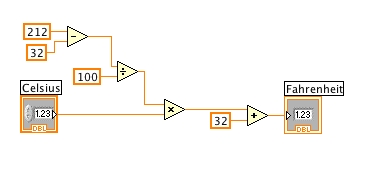
\includegraphics[height=2in]{graphical/C2F.jpg}
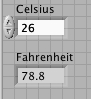
\includegraphics[height=2in]{graphical/C2FFP.jpg}
\caption{A LabVIEW-related graphic}
\label{fig-LabVIEWgraphic}
\end{figure}

%\begin{wrapfigure}[15]{r}{2in}
%\begin{center}
%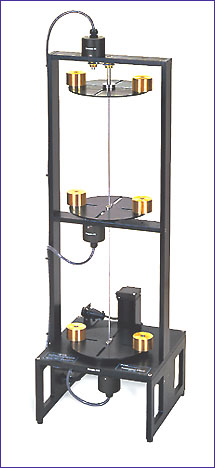
\includegraphics[height=4in]{Lab2/model205}
%\end{center}
%\caption{The ECP Torsional Disk System.}
%\label{fig-ecp}
%\end{wrapfigure}


%% Local Variables:
%% TeX-master: "../LVmanual.tex"
%% End:

